\chapter{Основы теории разработки программного обеспечения}

\section{Модели жизненного цикла программного обеспечения}

Базовым понятием в методологии проектирования программного обеспечения (ПО) можно назвать понятие жизненного цикла ее ПО. Жизненный цикл программного обеспечения (ЖЦ ПО) -- это определенные стадии, через которые проходит программное обеспечение от возникновения идеи до программной реализации с последующей поддержкой. Жизненный цикл заканчивается, в момент полного изъятия программного обеспечения из эксплуатации \cite{6, 22}.

Обычно, жизненный цикл представляют в виде различных моделей. Модель ЖЦ ПО --\: это структура, которая определяет последовательность выполнения и взаимосвязи процессов на различных этапах, на протяжении всего жизненного цикла. Модель ЖЦ ПО зависит от определенных параметров, которыми обладает ПО:
\begin{enumerate}
    \item [1)] специфика ПО;
    \item [2)] масштаб ПО;
    \item [3)] сложность проекта;
    \item [4)] специфика условий, в которых создается и функционирует ПО.
\end{enumerate}

Модель жизненного цикла отражает в себе различные состояния ПО, с момента возникновения необходимости в данном ПО до момента полного выхода из эксплуатации.

Далее представлены основные модели ЖЦ ПО, их описание, достоинства и недостатки, а также их особенности.

\subsection{Каскадная модель жизненного цикла программного обеспечения}

Основная суть каскадной модели заключается в том, что содержащиеся в ней этапы зависят друг от друга и следующий этап сможет начаться только тогда, когда закончен предыдущий, образуя таким образом последовательное движение вперед \cite{1, 19}.
В результате завершения всех этапов формируются промежуточные продукты, которые не могут изменяться на следующих этапах. Каскадная модель представлена на рисунке \ref{fig:1}.

\begin{figure}[h!]
    \center
    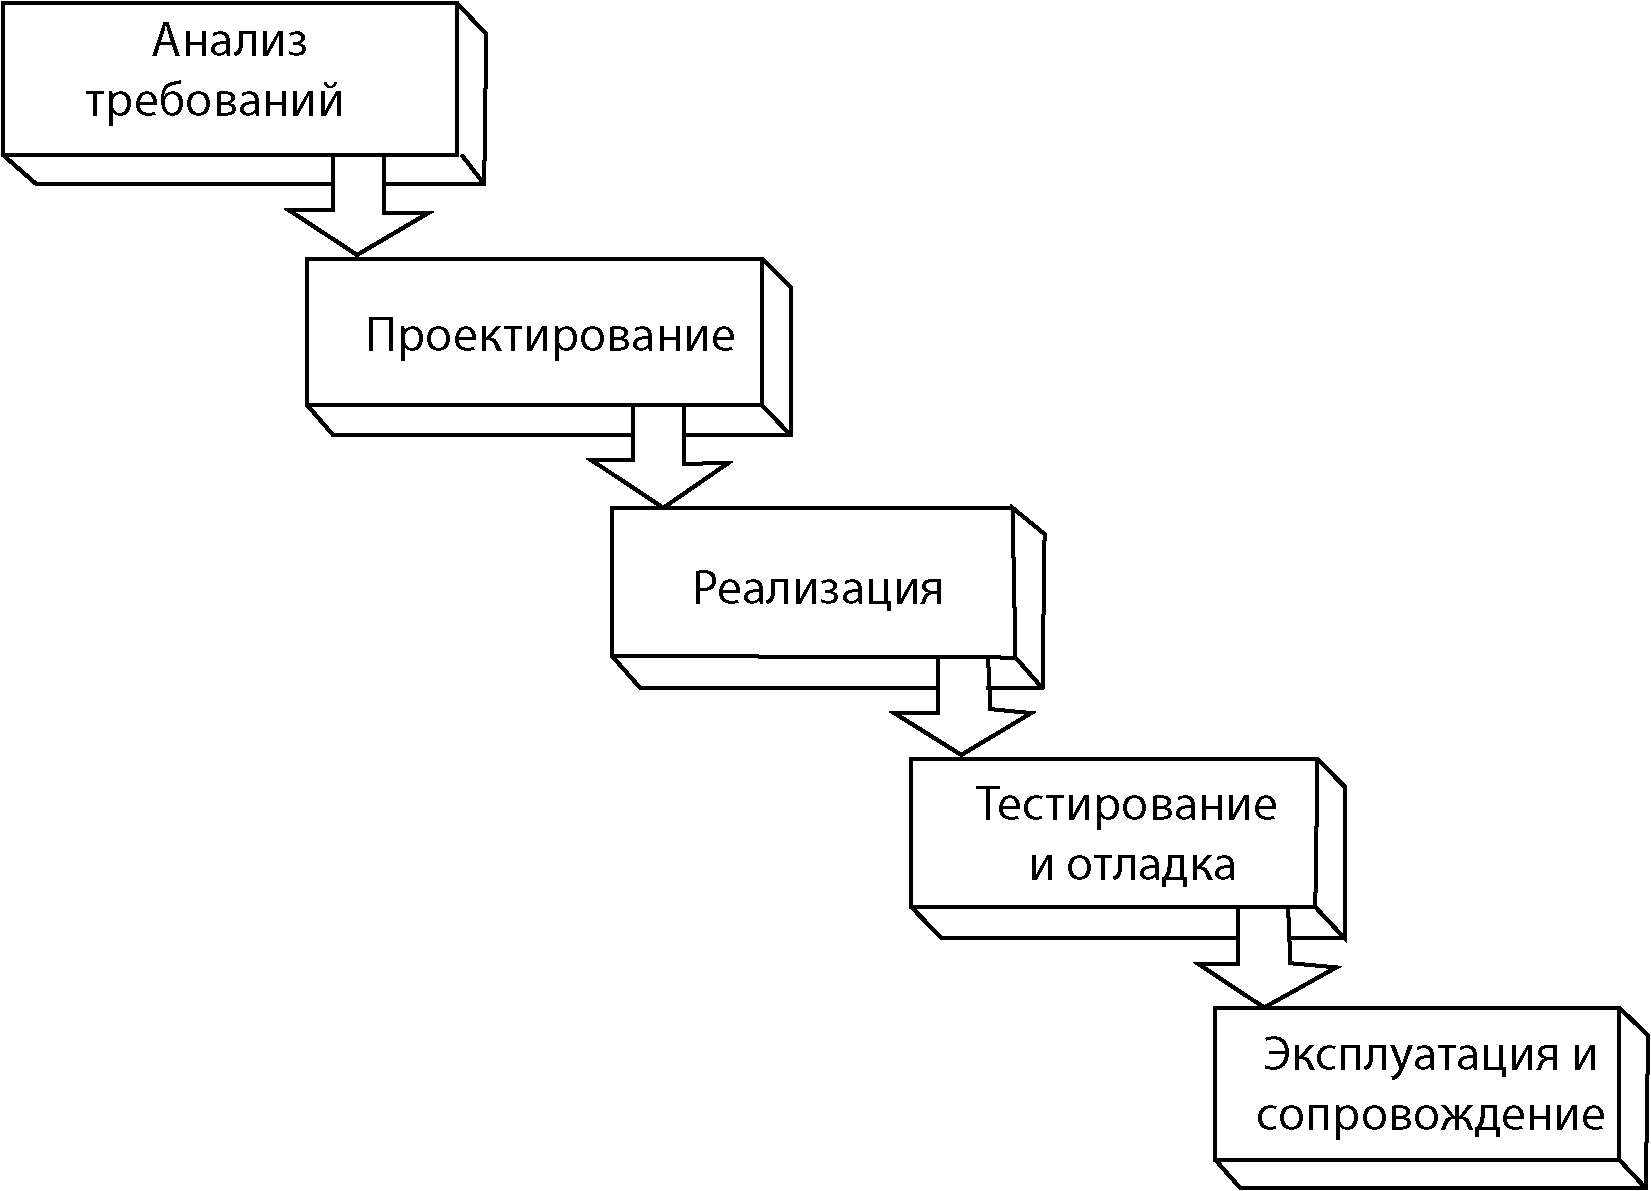
\includegraphics[scale=1]{fig/1.png}
    \caption{Каскадная модель ЖЦ ПО}
    \label{fig:1}
\end{figure}

Основные этапы каскадной модели: 
\begin{enumerate}
    \item [1)] анализ требований;
    \item [2)] проектирование;
    \item [3)] кодирование;
    \item [4)] тестирование и отладка;
    \item [5)] эксплуатация и сопровождение.
\end{enumerate}

Среди достоинств такой модели можно выделить:
\begin{enumerate}
    \item [1)] на каждой стадии формируется законченный набор документации, который выполняет критерии полноты и согласованости;
    \item [2)] простота и удобство в применении обусловлены тем, что процесс разработки такой модели выполняется поэтапно;
    \item [3)] так как шаги в этой модели осуществляются в логичной последовательности, можно запланировать сроки завершения всех этих шагов и соответствующие траты.
\end{enumerate}

К недостаткам каскадной модели относятся: 
\begin{enumerate}
    \item [1)] определение ошибок и недоработок на любом шаге, возможно только на следующих шагах;
    \item [2)] изменение каких-либо деталей в проекте возможно после того, как все этапы завершатся;
    \item [3)] промежуточный продукт, полученный такой моделью, будет непригоден для использования пользователями;
    \item [4)] трудность формулирования четких требований и отсутствие возможности динамически изменять их, на протяжении всего жизненного цикла;
    \item [5)] малое участие пользователя в создании системы, так как это возможно только на этапе разработки требований и в конце, когда система уже будет готова.
\end{enumerate}

Несмотря на все те минусы, которые есть у этой модели, она не ограничена только одной сферой применения, ее используют для решения таких типов задач, как научно-вычислительные, операционные системы и компиляторы, системы реального времени управления определенными объектами. Также каскадная модель может применяться при повторной разработке типового продукта, при выпуске новой версии существующей системы, если требования к вносимым изменениям четко определены \cite{23, 20}.

\subsection{Инкрементная модель жизненного цикла программного обеспечения}

Процесс разработки системы, при котором требования разбиваются на определенное количество отдельных модулей цикла разработки, является инкрементной моделью. Каждый такой шаг проходит определенные этапы, такие как этап требований, проектирования, кодирования и тестирования. Каждый выпуск системы может добавлять функцию к предыдущему выпуску, пока все разработанные функции не будут реализованы \cite{8, 9}. Первый выпуск системы часто оказывается основной рабочей системой, которую на последующих итерациях модернизируют и добавляют различный функционал. Инкрементная модель ЖЦ ПО представлена на рисунке \ref{fig:2}.

\begin{figure}[h!]
    \center
    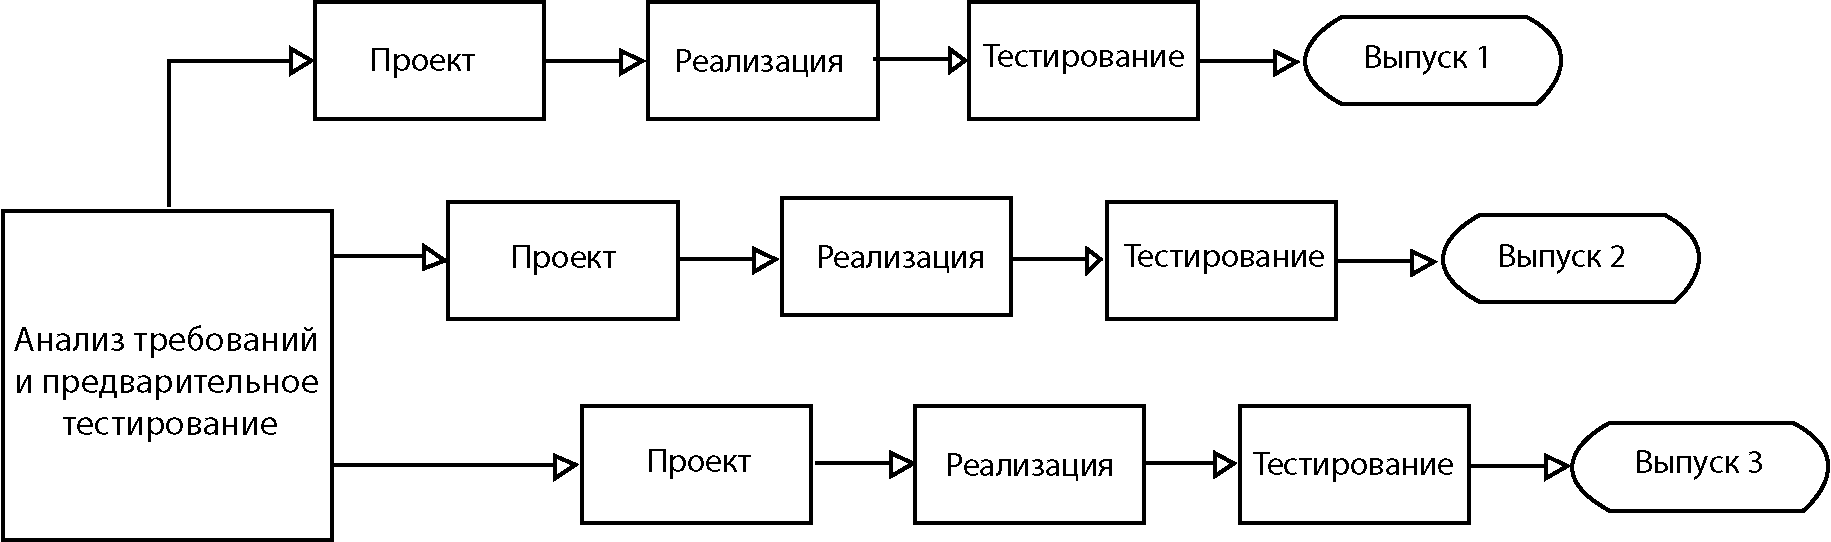
\includegraphics[scale=1]{fig/2.png}
    \caption{Инкрементная модель ЖЦ ПО}
    \label{fig:2}
\end{figure}

Основными преимуществами инкрементной модели являются: 

\begin{enumerate}
    \item [1)] система будет создаваться быстро в течении жизненного цикла программного обеспечения;
    \item [2)] на всех этапах разработки могут быть внесены изменения;
    \item [3)] стоимость разработки проекта гораздо ниже;
    \item [4)] клиент может вносить правки и изменения в течении всего процесса разработки;
    \item [5)] в такой модели проще идентифицировать ошибки.
\end{enumerate}

Также данная модель имеет следующие недостатки: 

\begin{enumerate}
    \item [1)] проблемы могут возникнуть из-за архитектуры системы, поэтому не все требования можно собрать заранее за весь жизненный цикл программного обеспечения;
    \item [2)] каждая фаза итерации жесткая и не перекрывает друг друга;
    \item [3)] устранение проблемы в одной единице требует исправления во всех единицах и занимает много времени.
\end{enumerate}

Инкрементные модели можно использовать в ряде случаев: когда требования системы четко ясны, когда возникает потребность в досрочном выпуске продукта, когда команда разработчиков ПО не очень хорошо подготовлена или обучена, когда задействованы функции и цели высокого риска. Данная методология чаще всего используется для веб-приложений и компаний на основе продуктов \cite{21}.

\subsection{Спиральная модель жизненного цикла программного обеспечения}

Спиральная модель основывается на итерационном процессе разработки, ее основной упор делается на начальные этапы ЖЦ, такими как анализ и проектирование, так именно здесь будут проверяться и обосновываться реализуемость технических решений путем создания прототипов (рисунок \ref{fig:3}). 

Схема работы такой модели очень проста, разработка вариантов системы представляется как набор циклов раскручивающейся спирали, каждому ее циклу соотвествует такое же количество стадий, как и в каскадной модели. Но начальные стадии, связанные с анализом и планированием, представленны более подробно с добавлением новых элементов \cite{13, 14}.

В каждом цикле выделяются четыре основные фазы: 

\begin{enumerate}
    \item [1)] определение целей, других вариантов и ограничений;
    \item [2)] оценка других вариантов, идентификация и разрешение рисков;
    \item [3)] разработка продукта следующего уровня;
    \item [4)] планирование следующей фазы.
\end{enumerate}

\begin{figure}[h!]
    \center
    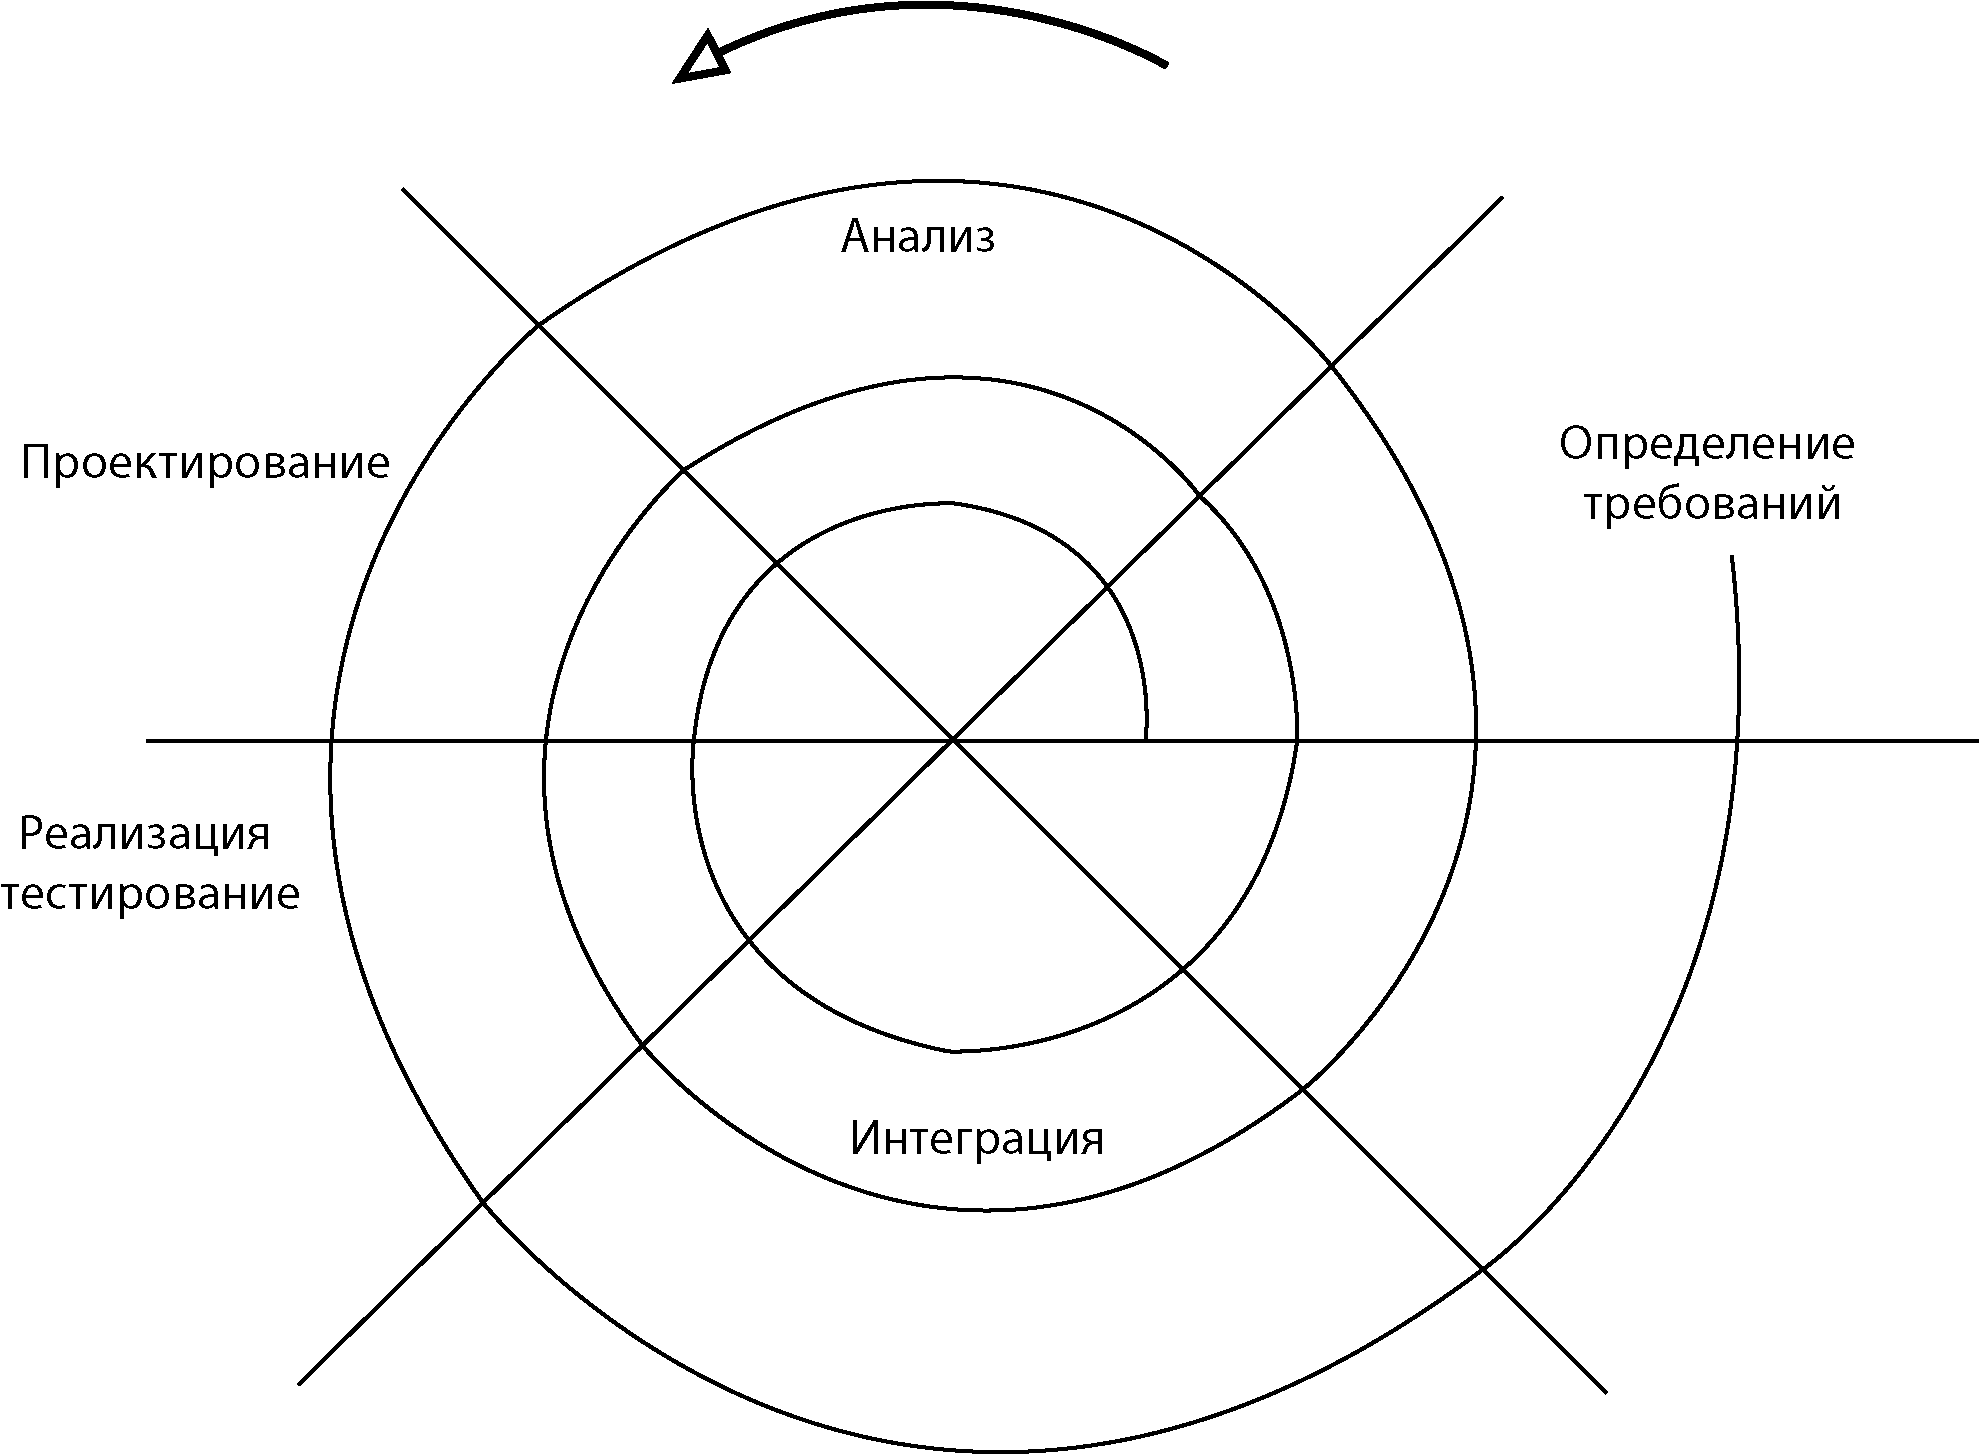
\includegraphics[scale=0.8]{fig/3.png}
    \caption{Спиральная модель ЖЦ ПО}
    \label{fig:3}
\end{figure}

Преимущества данной модели:

\begin{enumerate}
    \item [1)] проще внести изменения в систему при изменении требований заказчика;
    \item [2)] отдельные элементы системы интегрируются в единое целое постепенно, процесс интеграции производится практически непрерывно;
    \item [3)] уменьшается уровень рисков, так как они обнаруживаются именно в процессе интеграции;
    \item [4)] появляется гибкость в управлении проектом;
    \item [5)] итерационный подход упрощает повторное использование компонентов.
\end{enumerate}

Несмотря на все плюсы данной модели, у нее также имеется ряд недостатков: 

\begin{enumerate}
    \item [1)] сложность анализа и оценки  рисков при выборе вариантов;
    \item [2)] сложность поддержания версий системы (их хранение, возврат к ранним версиям);
    \item [3)] сложность оценки точки перехода на следующий цикл;
    \item [4)] бесконечность модели, так как на каждом витке заказчик может выдвигать новые требования, которые приводят к необходимости следующего цикла разработки.
\end{enumerate}

Данную модель лучше всего применять в случаях разработки проектов, использующих новые технологии, при разработке новой серии системы, при разработке систем, требующих демонстрации качества и версий системы через короткий период времени, при разработке систем для которых необходим подсчет затрат, связанных с оценкой и разрешением рисков. В этих задачах спиральная модель покажет все свои лучшие стороны и эффективно поможет разработать ту или иную систему \cite{26}. 

\section{Основные этапы разработки программного обеспечения}
В зависимости от модели жизненного цикла программного обеспечения количество и порядок этапов меняется, однако их задачи и проблемы, которые они решают одни для всех архитектур. Далее приведены основные этапы, присущие для любого вида разработки программного обеспечения.
\subsection{Анализ требований и разработка документации}
Первым этапом является формирование и анализ требований к программному продукту. В течении этого этапа важно определить рамки проекта, основываясь на ожиданиях заказчика. В результате анализа требований должно появится высокоуровневое описание сценариев работы системы, некоторая оценка затрат и рисков, возможных в ходе разработки. Все эти факторы формируют стоимость продукта и определяют количество необходимых ресурсов на разработку проекта. 

Функциональные и нефункциональные -- две разновидности требований. Функциональные описывают требуемую функциональность и различные особенности поведения системы. Нефункциональные описывают способы эксплуатации системы, например, требования к удобству использования, надежности, производительности и тому подобное \cite{17, 18}.
Функциональные требования -- это пользовательские сценарии, которые должны быть реализованы в системе. Если они работают так как нужно клиенту, то эти требования выполнены. 
Нефункциональные требования оформляются отдельно и должны учитывать экстремальные особенности которые должна выдерживать система. Одним из самых оптимальных способов выполнения нефункциональных требований на данный момент является использование веб-кластера, решающего задачи отказоустойчивости (дублирует несколько узлов), масштабируемости (можно добавлять сервера приложений и базы данных), надёжности (данные распределены по нескольким машинам) \cite{15, 16}.
\subsection{Прототипирование и моделирование теоретической основы}
Следующим этапом жизненого цикла программного обеспечение является проектирование теоретических моделей, общего плана работ, а также выбор технологий разработки. В ходе этого этапа формируются основные диаграммы в различных нотациях для визуализации процессов, поведение систем проекта, потоков данных, закладывается теоретический фундамент, являющийся основой для дальнейшей реализации \cite{4, 11}.

Проектирование разделяется на две разновидности: техническое и логическое. В процессе логического проектирования создается логическое представление данных в виде описания предметной области, объектов внутри нее, их характеристик и логических связей. В процессе технического проектирования расширяется логическое представления данных материальными характеристиками и наложением их функционала на функционал логических объектов. В результате процесса проектирования появляются функциональная и системная архитектура проекта.

\subsection{Реализация и тестирование программного обеспечения}

Этап реализации и тестирования является прямым продолжением предыдущих двух. В ходе реализации происходит кодирование основного функционала, создание всех описанных логических связей и оформление кода в формате, позволяющем дополнить и ркасширить его в дальнейшем. Тестирование -- важнейшая часть данного этапа. В процессе тестирования выявляются недоработки на предыдущих этапах, проверяется соответствие программного продукта техническомцу заданию и решаются ранее непредвиденные проблемы. Контроль качества продукта -- анализ результатов тестирования и качества новых версий выпускаемого продукта. Обеспечение качества продукта -- изучение возможностей по изменению и улучшению процесса разработки, улучшению коммуникаций в команде, где тестирование является только одним из аспектов обеспечения качества.Модульное тестирование (юнит-тестирование) -- тестируется минимально возможный для тестирования компонент, например, отдельный класс или функция. Часто модульное тестирование осуществляется разработчиками ПО \cite{10, 12}.

Тестирование программного продукта разбивается на уровни \cite{2, 3}.
Интеграционное тестирование -- тестируются интерфейсы между компонентами, подсистемами. При наличии резерва времени на данной стадии тестирование ведётся итерационно, с постепенным подключением последующих подсистем.
Системное тестирование -- тестируется интегрированная система на её соответствие требованиям.
Альфа-тестирование -- имитация реальной работы с системой штатными разработчиками, либо реальная работа с системой потенциальными пользователями/заказчиком. Чаще всего альфа-тестирование проводится на ранней стадии разработки продукта, но в некоторых случаях может применяться для законченного продукта в качестве внутреннего приёмочного тестирования. Иногда альфа-тестирование выполняется под отладчиком или с использованием окружения, которое помогает быстро выявлять найденные ошибки. Обнаруженные ошибки могут быть переданы тестировщикам для дополнительного исследования в окружении, подобном тому, в котором будет использоваться ПО \cite{5, 7}.
Бета-тестирование -- в некоторых случаях выполняется распространение версии с ограничениями (по функциональности или времени работы) для некоторой группы лиц, с тем чтобы убедиться, что продукт содержит достаточно мало ошибок. Иногда бета-тестирование выполняется для того, чтобы получить обратную связь о продукте от его будущих пользователей.




